Ce chapitre décrit les différents diagrammes d'intéraction.

\section{Fonctionnalité 1}
Ce paragraphe décrit les diagrammes d'intéraction concernant la fonctionnalité 1. \\

La figure suivant (figure \ref{diagrammeInteraction1}) indique le déroulement de la création, la modification et la suppression d'un bénévole par un administrateur.
\begin{figure}[H]
	\centering
	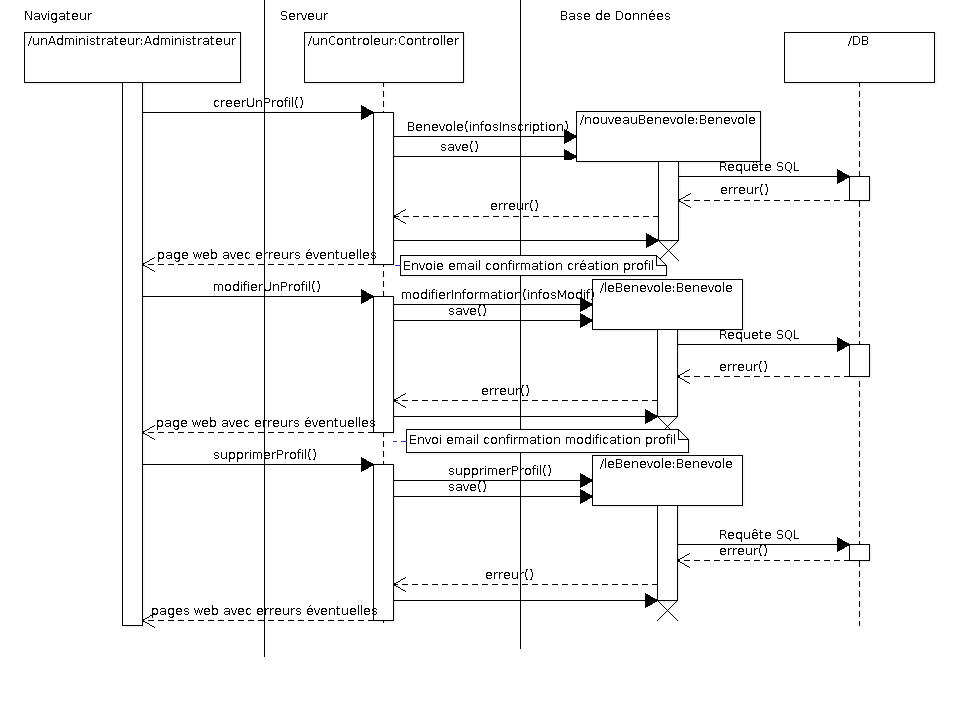
\includegraphics[scale=0.57]{images/diagrammesInteraction/01_diagrammeInteractionF1.png}
	\caption{Diagramme d'intéraction~: Création, modification, suppression d'un bénévole par un administrateur}
	\label{diagrammeInteraction1}
\end{figure}

La figure suivante (figure \ref{diagrammeInteraciton2}) indique le déroulement de la connexion et la déconnexion d'un bénévole.
\begin{figure}[H]
	\centering
	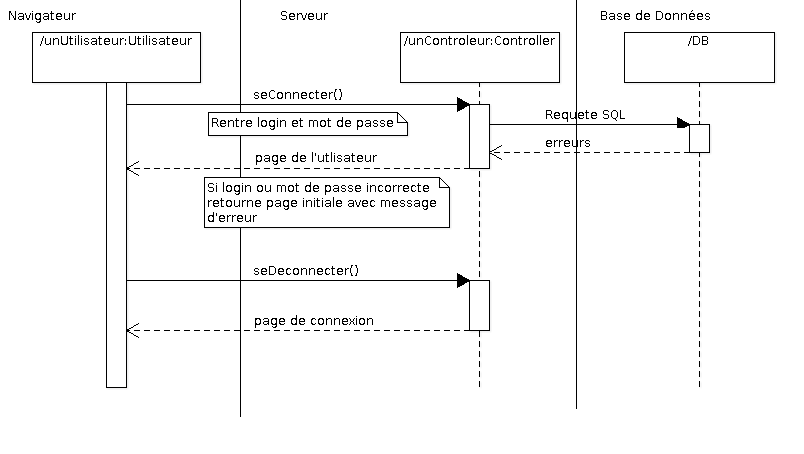
\includegraphics[scale=0.65]{images/diagrammesInteraction/02_diagrammeInteractionF1.png}
	\caption{Diagramme d'intéraction~: Connection et déconnection d'un utilisateur}
	\label{diagrammeInteraciton2}
\end{figure}

\section{Fonctionnalité 2}
Ce paragraphe décrit le diagramme d'intéraction concernant la fonctionnalité 2. \\

La figure suivante (figure \ref{diagrammeInteraction3}) indique le déroulement de la création, la modification et la suppression d'un établissement par un administrateur.
\begin{figure}[H]
	\centering
	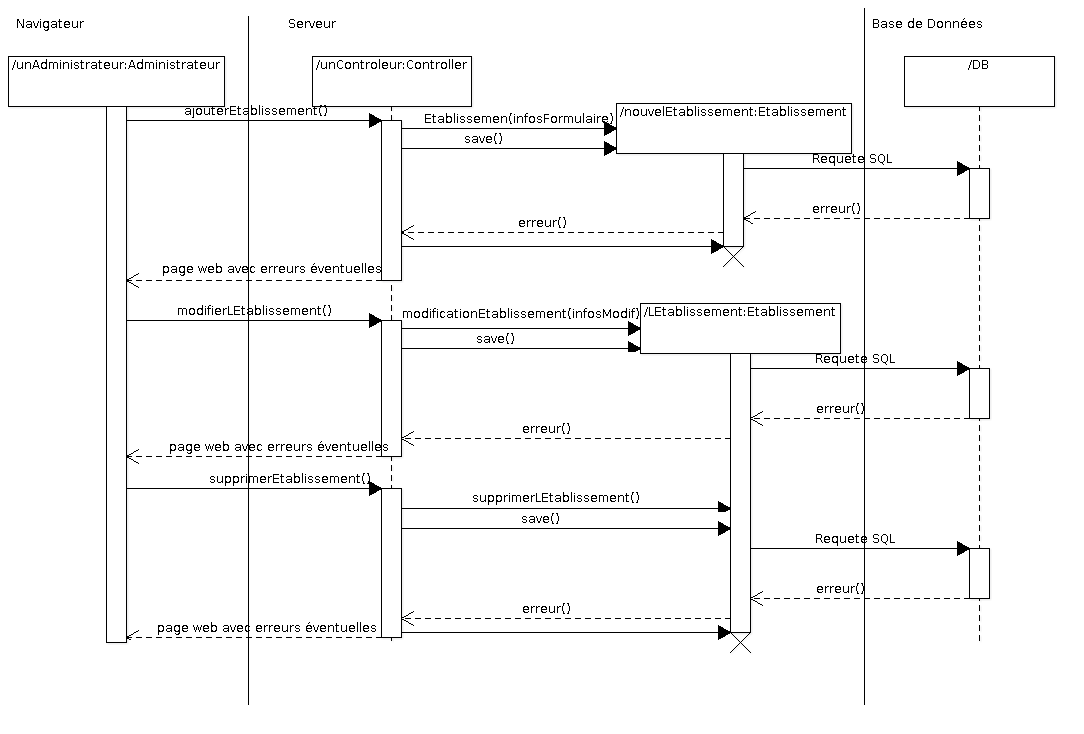
\includegraphics[scale=0.5]{images/diagrammesInteraction/03_diagrammeInteractionF2.png}
	\caption{Diagramme d'intéraction~: Création, modification, suppression d'un établissement par un administrateur}
	\label{diagrammeInteraction3}
\end{figure}

\section{Fonctionnalité 3}
Ce paragraphe décrit le diagramme d'intéraction concernant la fonctionnalité 3. \\

La figure suivante (figure \ref{diagrammeInteraction4}) indique le déroulement de l'envoi du formulaire de demande d'intervention aux établissements.
\begin{figure}[H]
	\centering
	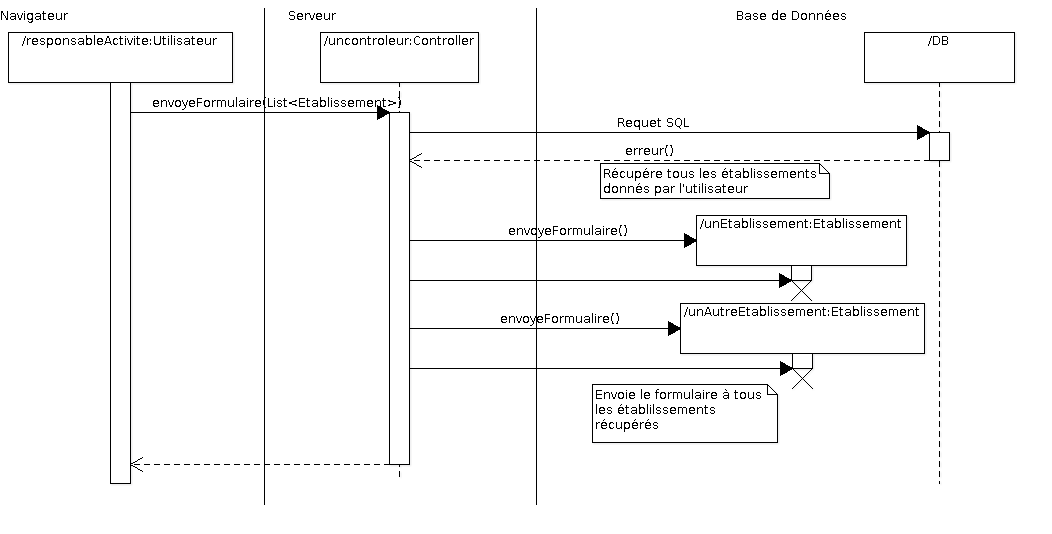
\includegraphics[scale=0.5]{images/diagrammesInteraction/04_diagrammeInteractionF3.png}
	\caption{Diagramme d'intéraction~: Envoye du formulaire à un ensemble d'établissement}
	\label{diagrammeInteraction4}
\end{figure}

\section{Fonctionnalité 4}
Ce paragraphe décrit les diagramme d'intéraction concernant la fonctionnalité 4. \\

La figure suivante (figure \ref{diagrammeInteraction5})
\begin{figure}
	\centering
	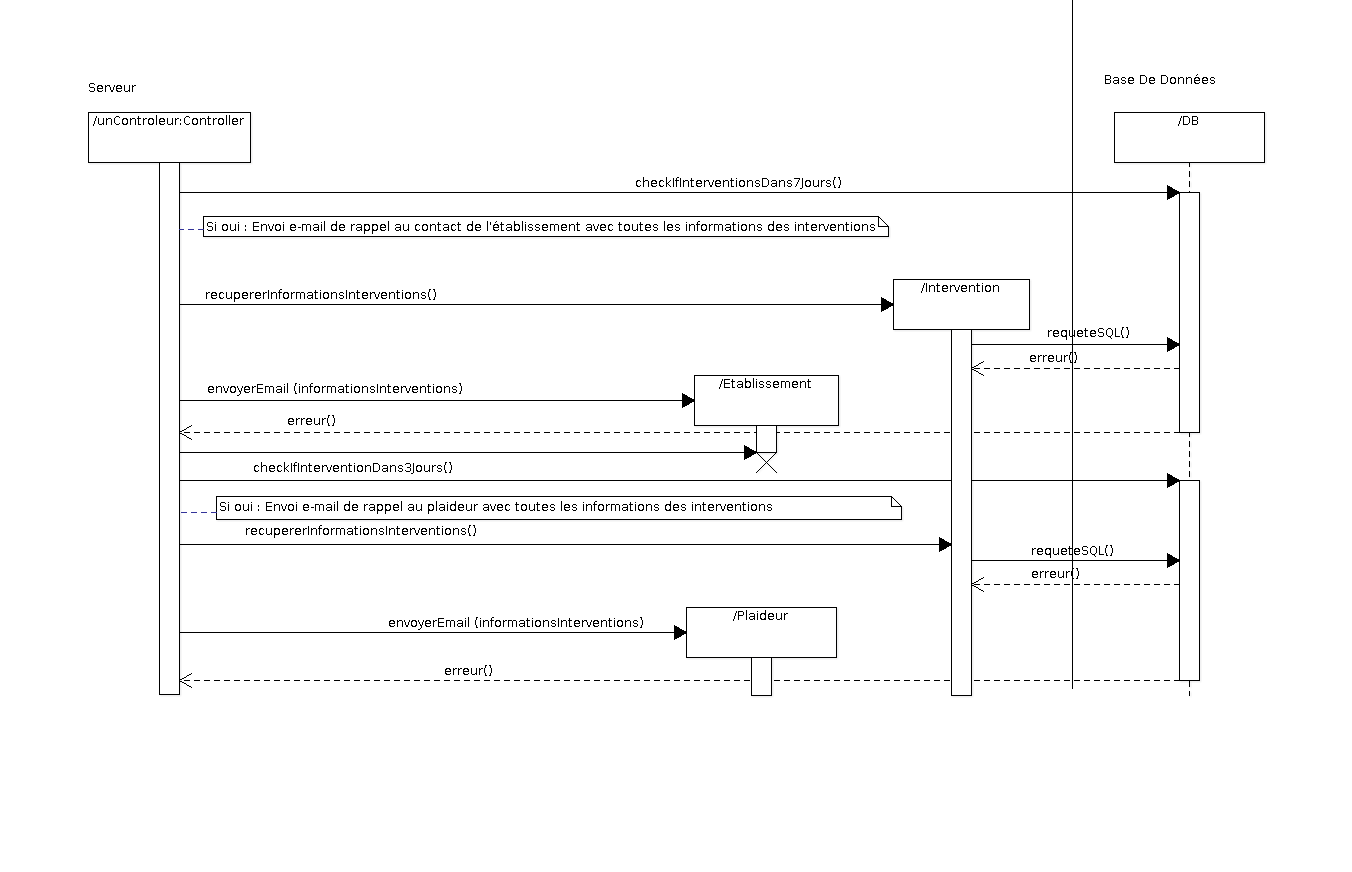
\includegraphics[scale=0.5]{images/diagrammesInteraction/05_diagrammeInteractionF4.png}
	\caption{Diagramme d'intéraction~: Replissage du formulaire}
	\label{diagrammeInteraction5}
\end{figure}